\documentclass[notes=hide,yellow]{beamer}

% (c) 2008 Steffen Klemer <moh AT gmx BEEP org>
% This work is licensed under the Creative Commons Attribution-Share Alike 3.0
% Germany License. To view a copy of this license, visit
% http://creativecommons.org/licenses/by-sa/3.0/de/ or send a letter to Creative
% Commons, 171 Second Street, Suite 300, San Francisco, California, 94105, USA.
%
% See http://www.noch-mehr-davon.de/vortr.shtml
% Permissions beyond the scope of this license may be available at the same site
%
% Template based on: Copyright 2004 by Till Tantau <tantau@users.sourceforge.net>.


\mode<presentation>
{
%	\usetheme{AnnArbor} %Szeged
%	\usetheme{Berkeley}
	\usetheme{Frankfurt}
%	\usecolortheme{rose} %oder beaver oder rose oder orchid, albatross, rose
% 	\useinnertheme{circles}
%	\useoutertheme{split}
%	\setbeamercovered{invisible} %or transparent
% 	\usefottheme{professionalfonts}
% 	\usefonttheme[onlymath]{serif}
        %\setbeamercovered{invisible}
%	\setbeamertemplate{navigation symbols}{}
}

\usepackage{amsmath,amssymb,latexsym}
\usepackage{fancyvrb}
\usepackage{graphicx}
\usepackage{epstopdf}
\usepackage{amsfonts}
\usepackage{amsthm}
\usepackage{wasysym}
\usepackage{ucs}
\usepackage{listings}
\usepackage{stmaryrd}
\usepackage{hyperref}
\usepackage{graphics}
\usepackage{colortbl}

\usepackage{tikz}
\tikzstyle{every picture}+=[remember picture]
\usetikzlibrary{arrows}
\usetikzlibrary{shadows}
\usetikzlibrary{fit}
\usetikzlibrary{shapes}
\usetikzlibrary{backgrounds}

\tikzstyle{vertex}=[circle,fill=black!25,minimum size=12pt,inner sep=0pt]
\tikzstyle{selected vertex} = [vertex, fill=red!24]
\tikzstyle{blue selected vertex} = [vertex, fill=blue!25]
\tikzstyle{edge} = [draw,thick,-]
\tikzstyle{weight} = [font=\small]
\tikzstyle{selected edge} = [draw,line width=5pt,-,red!50]
\tikzstyle{ignored edge} = [draw,line width=5pt,-,black!20]
\tikzstyle{small vertex}=[circle,fill=black!25,minimum size=8pt, inner sep=0pt]
\tikzstyle{small selected vertex}=[circle,fill=red!25,minimum size=8pt, inner sep=0pt]



%\usepackage[ngerman]{babel}
%\usepackage[utf8x]{inputenc}




\title{An overview of current BGP security problems}
\subtitle{ }
\author{Ralph Krimmel}



\begin{document}
	\begin{frame}
		\titlepage
	\end{frame}

	\begin{frame}
		\tableofcontents
	\end{frame}

\section{ Introduction}
\subsection*{}

\begin{frame}{Routing in the Internet}
	\begin{block}{The Internet}
	\begin{itemize}
		\item Large, decentralized Network %of smaller networks
		\item Intermediate hosts: Routers
		\item Internet protocol
	\end{itemize}
\end{block}
\end{frame}


\begin{frame}
	\frametitle{Some definitions}
	\begin{block}{IP Addresses}
	\begin{itemize}
		\item IP Address: 32(v4)/128(v6) bit Numbers
		\item E.g.: Host: 134.76.80.1  Subnet: 134.76.80.0/24
		\item IP Prefix: Block of IP addresses
	\end{itemize}
	\end{block}
	
\end{frame}

\begin{frame}
	\frametitle{Some definitions \#2}
	\begin{block}{Autonomous Systems}
	\begin{itemize}
		\item Collection of IP prefixes under control of one organisation
		\item Identified by \emph{AS Number}
			\begin{itemize}
				\item Public: 1-64511
				\item Private: 64512-65535 
			\end{itemize}
		\item Exchange routing information with adjacent autonomous systemss% on how to reach specific blocks of Prefixes
	\end{itemize}
	\end{block}
	
\end{frame}

\begin{frame}
	\frametitle{BGP}
	\begin{block}{BGP Basics}
		\begin{itemize}

			\item Incremental protocol
			\item 4 Message Types
				\begin{itemize}
					\item Open: Session initiation
					\item \textbf{Update}: Advertisement/withdrawal of routes
					\item Notification: Session termination
					\item Keepalive: Verification of reachability
				\end{itemize} 
	%	\item Path-Vector Protocol
		\end{itemize}
	\end{block}
\end{frame}


\begin{frame}
	\frametitle{BGP Update Message}
	\begin{block}{Important attributes}
	\begin{itemize}
		\item Next hop: Destination of the next hop router   
		\item AS-Path: Path with AS-Numbers leading to prefix 
		\item Several attributes for path selection (MED, Origin, Local preference)
	\end{itemize}
	\end{block}
\end{frame}

\begin{frame}
	\frametitle{Path selection}
	
	\begin{block}{Decision factors}
	\begin{enumerate}
		\item Local preference 
		\item Shortest AS path length
		\item Lowest origin value
		\item Lowest MED value
		\item ...
	\end{enumerate}
	\end{block}
\end{frame}

\begin{frame}{Example}
	\begin{center}
		\includegraphics[width=\textwidth]{example.pdf}
	\end{center}	
\end{frame}


\section{Security issues of BGP}
\subsection*{}
\begin{frame}
	\frametitle{Prefix hijacking}
		
	\begin{block}{No verification of:}
		\begin{itemize}
			\item Prefix ownership
			\item AS number ownership
		\end{itemize}
	\end{block}
\end{frame}

\begin{frame}{Short AS pathes}
	\begin{center}
		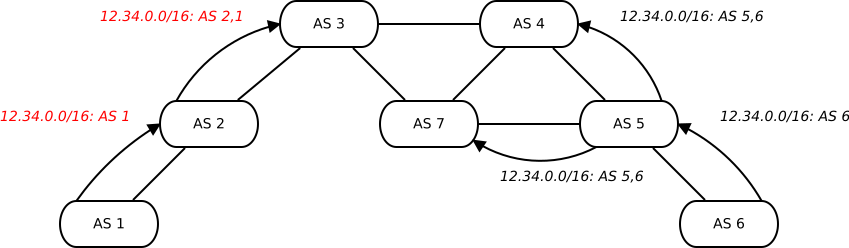
\includegraphics[width=\textwidth]{pathlength.pdf}
	\end{center}
\end{frame}

\begin{frame}{Deaggregation}
	\begin{center}
		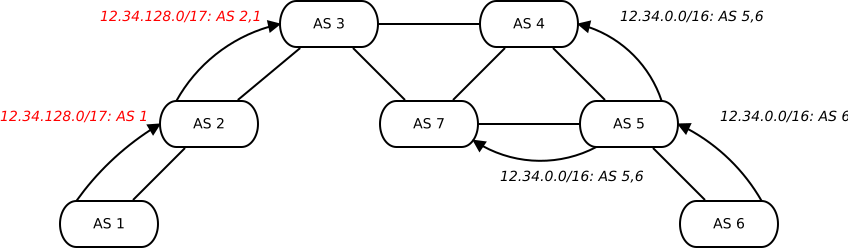
\includegraphics[width=\textwidth]{deaggregation.pdf}
	\end{center}
\end{frame}

\begin{frame}
	\frametitle{Attacks on TCP}
	
	\begin{block}{Attacks on TCP}
	\begin{itemize}
		\item Eavesdropping to learn routing information
		\item MITM: Insertion, modification and deletion of messages
		\item Replay attack
		\item DoS attacks (via RST, SYN-Flood)
	\end{itemize}
	\end{block}
\end{frame}


\section{Cryptographic techniques}
\subsection*{}


\begin{frame}{Cryptographig techniques}
	\begin{block}{Some techniques}
	\begin{itemize}
		\item Pairwise keying %shared secret
		\item Cryptographic hash functions (message digests) %\item Create fixed length output for variable input
		\begin{itemize} 
			\item Non-invertible
			\item Collision resistant
		\end{itemize}
		\item Message Authentication Code: digest(Shared key + Message) 
	\end{itemize}
	\end{block}
\end{frame}

\section{BGP security today}
\subsection*{}

\begin{frame}{BGP security today}
	\begin{block}{Current approaches}
	\begin{itemize}
		\item Protection of the BGP session between routers
		\item Defensive filtering
	\end{itemize}
	\end{block}
\end{frame}

\begin{frame}
	\frametitle{Protection of a BGP Session between routers}
	\begin{block}{Two goals}
	\begin{itemize}
		\item Protecting TCP 
		\item BGP session itself
	\end{itemize}
	\end{block}
\end{frame}


\begin{frame}
	\frametitle{Proposed solutions}
	\begin{block}{Countermeasures}
	\begin{itemize}
		\item MD5 Integrity
		\item Session and Message Protection
		\item Generalized TTL Securiy Mechanism
		\item IPsec
	\end{itemize}
	\end{block}
\end{frame}


\begin{frame}{MD5 Integrity}
	\begin{block}{Idea}
	\begin{itemize}
		\item TCP extension that uses a MAC based on MD5
		\item Carries MAC of TCP header and BGP data
	\end{itemize}
	\end{block}
	$\Rightarrow$ Protects integrity and prevents replay attacks
%%
\end{frame}
%
\begin{frame}{Session and Message Protection}
	\begin{block}{Proposed countermeasures}
	\begin{itemize}
		\item Adding sequence numbers
		\item Encryption of all BGP data between peers %shared secret
		\item Digital signatures of all UPDATE fields 
		%\item New path attribute: PREDECESSOR % identification of last AS before destination
	\end{itemize}
	\end{block}
	Disadvantages: BGP needs to be altered, based on shared keys
\end{frame}

\begin{frame}{Generalized TTL Security Mechanism}
	
	\begin{block}{Idea}
	\begin{itemize}
		\item IP header contains a TTL field 
		\item TTL decreased with every hop
		\item Utilize IP TTL to discard every packet with TTL $< 254$.
		\item Cheap solution
		\item Weakly defends against remote attacker
	\end{itemize}
	\end{block}
	%\begin{center}
%		\includegraphics[scale=0.3]{ttl.jpg}
%	\end{center}
	%=> Weakly defends against remote attacker, but not against malicious information coming from adjacent peers
	%=> Also, useless in multihop environments
\end{frame}
%
\begin{frame}{IPsec}
	\begin{block}{IPsec overview}
	\begin{itemize}
		\item IP layer protocol
		\item Three protocols: IKE (Key Managment, AH and ESP (packet level security)
		\item Provides: authenticy, integrity, replay prevention, confidentality, DOS prevention
		\item Widely used for securing BGP sessions
	\end{itemize}
	\end{block}
\end{frame}
%
\section{Defensive Filtering}
\subsection*{}

\begin{frame}{Defensive Filtering}
	Goal: Filter bad and potential malicious announcements
\end{frame}
\begin{frame}
%Usually ingress and egress filtering based on route policies like:
	\begin{block}{Route policies}
\begin{itemize}
	\item Prefixes with special uses
	\item Bogons %(Advertisements of address blocks and AS numbers with no matching allocation data, Black list needed
	\item Private AS numbers
	\item Long AS-Pathes
	\item Routes to small networks (Deaggreation prevention)
	\item Limit of announcements by a neighbour (DoS and Deaggreation prevention)
	\item Rewrite of BGP attributes
\end{itemize}
\end{block}
%%=> Filtering works basically well in practise but can not replace a strong security architecture
\end{frame}

\section{S-BGP}
\subsection*{}
\begin{frame}{S-BGP}
	\begin{block}{S-BGP overview}
		\begin{itemize}
			\item Full scale security architecture
			\item Installs PKI, parallel to existing allocation and delegation systems
			\item BGP data can be signed and verified
			\item IPsec to secure peer sessions
			\item Two kind of attestations: Address and route attestations
		\end{itemize}
	\end{block}
\end{frame}


\begin{frame}{Address attestations}
%The ownership of a prefix is checked by an out of band mechanism called Adress attestations by the validation of a delegation chain (similar to x509 PKI)
	\begin{block}{Address attestations}
	\begin{itemize}
		\item Out-of-band mechanism
		\item Verification of the ownership of prefixes via certificates
		\item Delegation chain, similar to x.509 PKI
	\end{itemize}
	\end{block}

\end{frame}

\begin{frame}{Route attestations}
	\begin{block}{Route attestations}
	\begin{itemize}
		\item Distributed via BGP
		\item Update messages can carry digital signatures %those authenticate an autonomous system
		\item Each AS in the path signes the path recursively 
	\end{itemize}
	\end{block}
\end{frame}

\begin{frame}{Route attestations}
			\begin{center}
				\includegraphics[scale=1.337]{sbgp.png}
			\end{center}
\end{frame}


\begin{frame}{Deployment issues}
	
	\begin{itemize}
		\item S-BGP needs more memory

		\item Alot of parties have to work together (IANA/ICANN)/ISPs/Router vendors
	\end{itemize}
\end{frame}


\begin{frame}{Summary}
	\begin{block}{Summary}
	\begin{itemize}
	\item BGP plays a large role in in internet routing
	\item BGP is vulnerable at many places
	\item Several existing practises to defend against threads
	\item Existing solutions are hard to deploy
	\end{itemize}
	\end{block}
\end{frame}

\begin{frame}
	\begin{center}
	\large Questions?
\end{center}
	\begin{center}
	\includegraphics[scale=0.8]{questions.jpg}
	\end{center}
\end{frame}
\end{document}


